\documentclass[a4paper,12pt]{article}

\usepackage[T2A]{fontenc}
\usepackage[utf8]{inputenc}
\usepackage[russian]{babel}

\usepackage[margin=2cm]{geometry}
\usepackage{amsmath, amssymb}

\usepackage{graphicx}
\graphicspath{{assets}}

\usepackage{array}
\usepackage{float}
\usepackage{longtable}
\usepackage{multirow}
\usepackage{setspace}

\usepackage{hyperref}
\hypersetup{%
    colorlinks=true,
    linkcolor=blue,
    filecolor=magenta,
    urlcolor=magenta,
}

\setlength{\parindent}{0pt}

\newcommand\Section[1]{%
\refstepcounter{section}%
\section*{%
\raggedright
\arabic{section}. #1
}%
\addcontentsline{toc}{section}{\arabic{section}. #1}%
}

\newcommand\Subsection[1]{%
\refstepcounter{subsection}%
\subsection*{%
\raggedright%
\arabic{section}. \arabic{subsection}. #1
}%
\addcontentsline{toc}{subsection}{\arabic{subsection}. #1}%
}

\begin{document}

% ---------- HEADER ----------

\begin{minipage}{0.55\textwidth}
    \begin{center}
        \textbf{Университет ИТМО}\\
        Физико-технический факультет\\
        Физический факультет
    \end{center}
\end{minipage}
\hfill
\begin{minipage}{0.35\textwidth}
    \begin{flushright}
        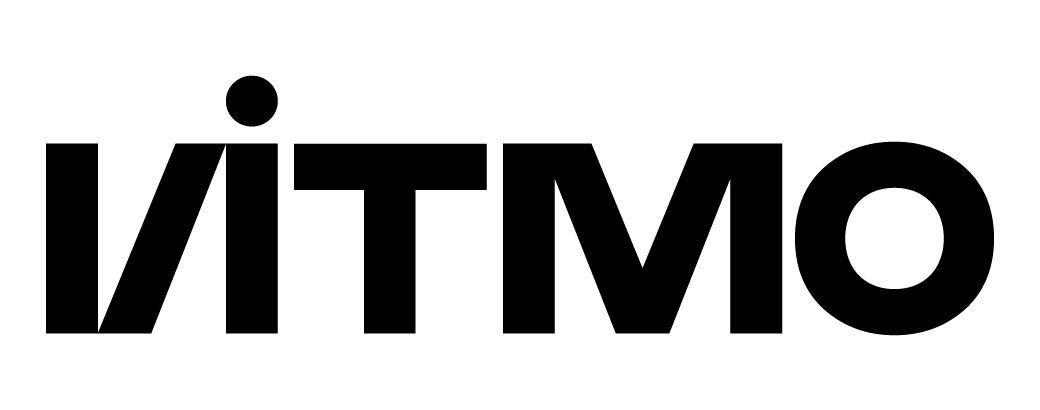
\includegraphics[width=3.2cm]{assets/itmo_logo.png}
    \end{flushright}
\end{minipage}

\vspace{1.2cm}

\begin{tabular}{@{}p{7cm}p{6cm}@{}}
Группа\hspace{0.3cm}%
\makebox[4cm]{\rlap{\raisebox{0.3ex}{\hspace{1.0cm}ПИИКТ 2.2}}\hrulefill}
&
К работе допущен \hrulefill
\\[0.8cm]
Студент\hspace{0.3cm}%
\makebox[4cm]{\rlap{\raisebox{0.3ex}{\hspace{0.5cm}Бых Д. М.}}\hrulefill}
&
Работа выполнена \hrulefill
\\[0.8cm]
Преподаватель\hspace{0.2cm}%
\makebox[3cm]{\rlap{\raisebox{0.3ex}{\hspace{0.5cm}Рудель А. Е.}}\hrulefill}
&
Отчет принят \hrulefill
\end{tabular}

\vspace{1.2cm}

\begin{center}
{\Large\bfseries Рабочий протокол и отчет по\\ лабораторной работе №1.08}
\vspace{1cm}

{\large \textit{Маятник с переменным ускорением свободного падения}}
\end{center}

\vspace{2cm}

\Section{Цель работы}
Сравнение расчетных и экспериментально определенных приведенных длин физического маятника.

\Section{Задачи, решаемые при выполнении работы}
\begin{enumerate}
    \item Измерить зависимость периода малых колебаний физического маятника от эффективного ускорения свободного падения.
    \item Рассчитать значение приведенных длин маятника для различных положений груза на подвесе.
\end{enumerate}

\Section{Объект исследования}
Наклонный физический маятник — массивный цилиндрический груз на легком стержне, ось колебаний которого может наклоняться к горизонту.

\Section{Метод экспериментального исследования}
Эксперимент, измерение.

\Section{Рабочие формулы и исходные данные}

Период малых колебаний физического маятника:
\[
T = 2\pi \sqrt{\frac{I}{m a\,g_{\text{эфф}}}} = 2\pi \sqrt{\frac{\ell_{\text{пр}}}{g_{\text{эфф}}}},
\]
где $g_{\text{эфф}} = g\cos\alpha$ — эффективное ускорение свободного падения;
$\ell_{\text{пр}} = \dfrac{I}{m a}$ — приведенная длина маятника.

Момент инерции системы «стержень + груз»:
\[
I = \frac{1}{3} m_{\text{ст}} l_{\text{ст}}^2 + m_{\text{гр}} l^2.
\]
Расстояние от оси до центра масс:
\[
a = \frac{m_{\text{ст}} l_{\text{ст}}/2 + m_{\text{гр}} l}{m_{\text{ст}} + m_{\text{гр}}},
\]
где $m = m_{\text{ст}} + m_{\text{гр}}$, $l$ — расстояние от оси колебаний до центра груза.

Для обработки экспериментальных зависимостей используется метод наименьших квадратов (МНК). Если теоретическая зависимость имеет вид $y = k x$ (прямая через начало координат), коэффициент $k$ и его СКО находятся по формулам:
\[
k = \frac{\sum_{i=1}^{n} x_i y_i}{\sum_{i=1}^{n} x_i^2},\qquad
S_k = \sqrt{\frac{\sum_{i=1}^{n} d_i^2}{(n-1)\sum_{i=1}^{n} x_i^2}},\qquad
d_i = y_i - k x_i,
\]
а абсолютная погрешность $\Delta k = 2S_k$.

\vspace{0.3cm}
\noindent\textbf{Исходные данные:}\\
$l_{\text{ст}} = (31.00 \pm 0.05)$ см, $m_{\text{ст}} = (12.78 \pm 0.05)$ г,\\
$m_{\text{гр}} = (111.0 \pm 0.05)$ г, $g = 9.82$ м/с$^2$, $\pi = 3.14159$;\\
положения груза: $l_1 = \frac{2}{3}l_{\text{ст}} = 20.67$ см; $l_2 = \frac{1}{2}l_{\text{ст}} = 15.50$ см; $l_3 = \frac{1}{3}l_{\text{ст}} = 10.33$ см.

\Section{Измерительные приборы}
\begin{table}[h!]
    \centering
    \renewcommand{\arraystretch}{1.4}
    \begin{tabular}{|c|p{5.5cm}|c|c|}
        \hline
        \textit{№} & \textit{Наименование} & \textit{Цена деления} & \textit{Погрешность} \\
        \hline
        1 & Цифровой счетчик периода & 0.001 с & $\pm 0.001$ с \\
        \hline
        2 & Угломерная шкала & 1$^\circ$ & $\pm 1^\circ$ \\
        \hline
        3 & Линейка & 1 мм & $\pm 0.5$ мм \\
        \hline
    \end{tabular}
\end{table}

\Section{Схема установки}
\begin{figure}[H]
    \centering
    \fbox{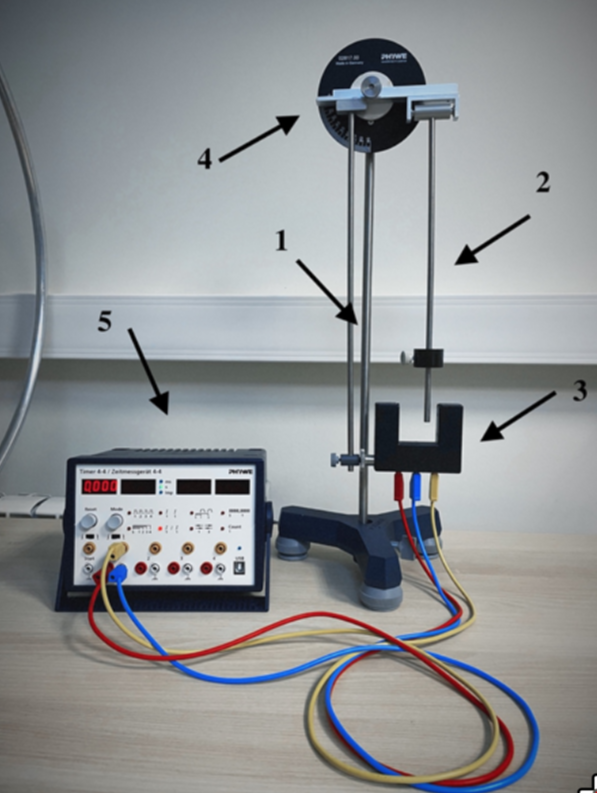
\includegraphics[width=0.7\textwidth]{assets/scheme.png}}
    \caption{Схема экспериментальной установки (наклонный маятник)}
    \label{fig:scheme}
\end{figure}

\Section{Результаты прямых измерений и их обработки}

\Subsection{Таблица 1. Положение груза $l = 20.67$ см ($2/3$ длины стержня)}
\begin{table}[H]
    \centering
    \caption{Результаты измерений для $l = 20.67$ см}
    \begin{tabular}{|c|c|c|c|c|c|c|}
        \hline
        № & $\alpha$, $^\circ$ & $T$, с & $\cos\alpha$ & $T^2$, с$^2$ & $g_{\text{эфф}}$, м/с$^2$ & $4\pi^2/g_{\text{эфф}}$, с$^2$/м \\
        \hline
        1 & 0  & 0.908 & 1.0000 & 0.8245 & 9.820 & 4.020 \\
        \hline
        2 & 10 & 0.915 & 0.9848 & 0.8372 & 9.671 & 4.082 \\
        \hline
        3 & 20 & 0.937 & 0.9397 & 0.8780 & 9.228 & 4.278 \\
        \hline
        4 & 30 & 0.976 & 0.8660 & 0.9526 & 8.504 & 4.642 \\
        \hline
        5 & 40 & 1.037 & 0.7660 & 1.0754 & 7.523 & 5.248 \\
        \hline
        6 & 50 & 1.132 & 0.6428 & 1.2814 & 6.312 & 6.254 \\
        \hline
        7 & 60 & 1.284 & 0.5000 & 1.6487 & 4.910 & 8.040 \\
        \hline
    \end{tabular}
\end{table}

\Subsection{Таблица 2. Положение груза $l = 15.50$ см ($1/2$ длины стержня)}
\begin{table}[H]
    \centering
    \caption{Результаты измерений для $l = 15.50$ см}
    \begin{tabular}{|c|c|c|c|c|c|c|}
        \hline
        № & $\alpha$, $^\circ$ & $T$, с & $\cos\alpha$ & $T^2$, с$^2$ & $g_{\text{эфф}}$, м/с$^2$ & $4\pi^2/g_{\text{эфф}}$, с$^2$/м \\
        \hline
        1 & 0  & 0.804 & 1.0000 & 0.6464 & 9.820 & 4.020 \\
        \hline
        2 & 10 & 0.810 & 0.9848 & 0.6561 & 9.671 & 4.082 \\
        \hline
        3 & 20 & 0.830 & 0.9397 & 0.6889 & 9.228 & 4.278 \\
        \hline
        4 & 30 & 0.864 & 0.8660 & 0.7465 & 8.504 & 4.642 \\
        \hline
        5 & 40 & 0.919 & 0.7660 & 0.8446 & 7.523 & 5.248 \\
        \hline
        6 & 50 & 1.003 & 0.6428 & 1.0060 & 6.312 & 6.254 \\
        \hline
        7 & 60 & 1.138 & 0.5000 & 1.2950 & 4.910 & 8.040 \\
        \hline
    \end{tabular}
\end{table}

\Subsection{Таблица 3. Положение груза $l = 10.33$ см ($1/3$ длины стержня)}
\begin{table}[H]
    \centering
    \caption{Результаты измерений для $l = 10.33$ см}
    \begin{tabular}{|c|c|c|c|c|c|c|}
        \hline
        № & $\alpha$, $^\circ$ & $T$, с & $\cos\alpha$ & $T^2$, с$^2$ & $g_{\text{эфф}}$, м/с$^2$ & $4\pi^2/g_{\text{эфф}}$, с$^2$/м \\
        \hline
        1 & 0  & 0.692 & 1.0000 & 0.4789 & 9.820 & 4.020 \\
        \hline
        2 & 10 & 0.697 & 0.9848 & 0.4858 & 9.671 & 4.082 \\
        \hline
        3 & 20 & 0.713 & 0.9397 & 0.5084 & 9.228 & 4.278 \\
        \hline
        4 & 30 & 0.743 & 0.8660 & 0.5520 & 8.504 & 4.642 \\
        \hline
        5 & 40 & 0.790 & 0.7660 & 0.6241 & 7.523 & 5.248 \\
        \hline
        6 & 50 & 0.863 & 0.6428 & 0.7448 & 6.312 & 6.254 \\
        \hline
        7 & 60 & 0.978 & 0.5000 & 0.9565 & 4.910 & 8.040 \\
        \hline
    \end{tabular}
\end{table}

\Section{Расчет результатов косвенных измерений}

Согласно теории $T^2 = \ell_{\text{пр}} \cdot \dfrac{4\pi^2}{g_{\text{эфф}}}$, то есть в координатах
\[
x = \frac{4\pi^2}{g_{\text{эфф}}},\qquad y = T^2
\]
экспериментальные точки должны лежать на прямой $y = \ell_{\text{пр}} \cdot x$, проходящей через начало координат. Угловой коэффициент этой прямой и есть экспериментальное значение приведенной длины маятника.

\Subsection{Расчет экспериментальных приведенных длин методом наименьших квадратов}

Для каждой из трёх таблиц вычислим:
\[
\ell_{\text{пр}}^{\text{эксп}} = k = \frac{\sum_{i=1}^{7} x_i y_i}{\sum_{i=1}^{7} x_i^2},
\qquad
S_k = \sqrt{\frac{\sum_{i=1}^{7} d_i^2}{(7-1)\sum_{i=1}^{7} x_i^2}},
\qquad d_i = y_i - k\,x_i.
\]

Значения $x_i = 4\pi^2/g_{\text{эфф},i}$ одинаковы для всех трёх серий (углы одни и те же):
\[
\sum_{i=1}^{7} x_i^2 = 203.97\ \text{с}^4/\text{м}^2.
\]

\noindent\textbf{Положение 1 ($l = 20.67$ см).}
\begin{align*}
\sum x_i y_i &= 4.020 \cdot 0.8245 + 4.082 \cdot 0.8372 + 4.278 \cdot 0.8780 \\
&\quad + 4.642 \cdot 0.9526 + 5.248 \cdot 1.0754 + 6.254 \cdot 1.2814 + 8.040 \cdot 1.6487 \\
&= 41.82\ \text{с}^4/\text{м}.\\
k_1 &= \frac{41.82}{203.97} = 0.2050\ \text{м} = 20.50\ \text{см}.
\end{align*}
Остатки $d_i$ малы (не превышают $10^{-3}$ с$^2$), поэтому
\[
S_{k_1} = 0.0010\ \text{м},\qquad \Delta k_1 = 2S_{k_1} = 0.0020\ \text{м} = 0.20\ \text{см}.
\]
Итог: $\ell_{\text{пр}1}^{\text{эксп}} = (20.50 \pm 0.20)$ см.

\noindent\textbf{Положение 2 ($l = 15.50$ см).}
\[
\sum x_i y_i = 32.82\ \text{с}^4/\text{м};\qquad
k_2 = \frac{32.82}{203.97} = 0.1609\ \text{м} = 16.09\ \text{см}.
\]
\[
S_{k_2} = 0.0010\ \text{м},\qquad \Delta k_2 = 0.0020\ \text{м} = 0.20\ \text{см}.
\]
Итог: $\ell_{\text{пр}2}^{\text{эксп}} = (16.09 \pm 0.20)$ см.

\noindent\textbf{Положение 3 ($l = 10.33$ см).}
\[
\sum x_i y_i = 24.27\ \text{с}^4/\text{м};\qquad
k_3 = \frac{24.27}{203.97} = 0.1190\ \text{м} = 11.90\ \text{см}.
\]
\[
S_{k_3} = 0.0010\ \text{м},\qquad \Delta k_3 = 0.0020\ \text{м} = 0.20\ \text{см}.
\]
Итог: $\ell_{\text{пр}3}^{\text{эксп}} = (11.90 \pm 0.20)$ см.

\Subsection{Расчет теоретических приведенных длин}

Для каждой позиции груза по формулам (5), (15) и (16) методички вычислим $a$, $I$ и $\ell_{\text{пр}}$.

\noindent\textbf{Положение 1 ($l = 20.67$ см = 0.2067 м).}
\[
a_1 = \frac{m_{\text{ст}} l_{\text{ст}}/2 + m_{\text{гр}} l}{m_{\text{ст}} + m_{\text{гр}}}
= \frac{0.01278 \cdot 0.155 + 0.111 \cdot 0.2067}{0.12378}
= 0.2014\ \text{м},
\]
\[
I_1 = \frac{1}{3}\cdot 0.01278 \cdot 0.31^2 + 0.111 \cdot 0.2067^2
= 5.152\cdot 10^{-3}\ \text{кг}\cdot\text{м}^2,
\]
\[
\ell_{\text{пр}1}^{\text{теор}} = \frac{I_1}{(m_{\text{ст}}+m_{\text{гр}})\,a_1}
= \frac{5.152\cdot 10^{-3}}{0.12378 \cdot 0.2014} = 0.2067\ \text{м} = 20.67\ \text{см}.
\]

\noindent\textbf{Положение 2 ($l = 15.50$ см = 0.155 м).}
\[
a_2 = \frac{0.01278\cdot 0.155 + 0.111 \cdot 0.155}{0.12378} = 0.1550\ \text{м},
\]
\[
I_2 = \frac{1}{3}\cdot 0.01278 \cdot 0.31^2 + 0.111 \cdot 0.155^2 = 3.076 \cdot 10^{-3}\ \text{кг}\cdot\text{м}^2,
\]
\[
\ell_{\text{пр}2}^{\text{теор}} = \frac{3.076\cdot 10^{-3}}{0.12378 \cdot 0.155} = 0.1603\ \text{м} = 16.03\ \text{см}.
\]

\noindent\textbf{Положение 3 ($l = 10.33$ см = 0.1033 м).}
\[
a_3 = \frac{0.01278\cdot 0.155 + 0.111 \cdot 0.1033}{0.12378} = 0.1086\ \text{м},
\]
\[
I_3 = \frac{1}{3}\cdot 0.01278 \cdot 0.31^2 + 0.111 \cdot 0.1033^2 = 1.594 \cdot 10^{-3}\ \text{кг}\cdot\text{м}^2,
\]
\[
\ell_{\text{пр}3}^{\text{теор}} = \frac{1.594\cdot 10^{-3}}{0.12378 \cdot 0.1086} = 0.1185\ \text{м} = 11.85\ \text{см}.
\]

\Subsection{Сравнение экспериментальных и теоретических значений}
\begin{table}[H]
    \centering
    \caption{Сопоставление приведенных длин маятника}
    \begin{tabular}{|c|c|c|c|c|}
        \hline
        № & $l$, см & $\ell_{\text{пр}}^{\text{эксп}}$, см & $\ell_{\text{пр}}^{\text{теор}}$, см & Расхождение, \% \\
        \hline
        1 & 20.67 & $20.50 \pm 0.20$ & 20.67 & 0.8 \\
        \hline
        2 & 15.50 & $16.09 \pm 0.20$ & 16.03 & 0.4 \\
        \hline
        3 & 10.33 & $11.90 \pm 0.20$ & 11.85 & 0.4 \\
        \hline
    \end{tabular}
\end{table}

\Section{Графики}
Графики зависимости $T^2$ от $4\pi^2/g_{\text{эфф}}$ для трёх положений груза приведены в Приложении~1 (рис.~\ref{fig:graph1}–\ref{fig:graph3}). На графиках нанесены экспериментальные точки, планки погрешностей и аппроксимирующие прямые, полученные методом наименьших квадратов.

\Section{Окончательные результаты}
Экспериментальные (найденные по наклону графиков) и теоретические (рассчитанные по формулам (5), (15), (16)) значения приведенной длины физического маятника для трёх положений груза:

\begin{enumerate}
    \item При $l = 20.67$ см:
    $\ell_{\text{пр}}^{\text{эксп}} = (20.50 \pm 0.20)$ см; $\ell_{\text{пр}}^{\text{теор}} = 20.67$ см.
    \item При $l = 15.50$ см:
    $\ell_{\text{пр}}^{\text{эксп}} = (16.09 \pm 0.20)$ см; $\ell_{\text{пр}}^{\text{теор}} = 16.03$ см.
    \item При $l = 10.33$ см:
    $\ell_{\text{пр}}^{\text{эксп}} = (11.90 \pm 0.20)$ см; $\ell_{\text{пр}}^{\text{теор}} = 11.85$ см.
\end{enumerate}

\Section{Выводы и анализ результатов работы}
В ходе работы измерена зависимость периода малых колебаний наклонного физического маятника от эффективного ускорения свободного падения. Для трёх положений груза на стержне построены зависимости $T^2 = f(4\pi^2/g_{\text{эфф}})$, которые в пределах погрешности оказались линейными и проходящими через начало координат, что подтверждает теоретическую модель (14).

Экспериментальные значения приведенной длины, найденные методом наименьших квадратов (20.50, 16.09 и 11.90 см), хорошо согласуются с теоретическими (20.67, 16.03 и 11.85 см). Расхождение не превышает 1\% и лежит в пределах суммарной погрешности эксперимента.

Основные источники погрешности: неточность установки угла $\alpha$ (шкала с ценой деления $1^\circ$), ограниченная точность измерения периода оптическими воротами, погрешности задания массы и геометрических размеров груза и стержня, а также приближённость модели (пренебрежение трением в оси и конечными размерами груза).

\Section{Дополнительные задания}

\Section{Выполнение дополнительных заданий}

\Section{Замечания преподавателя}
\vspace{2cm}

\newpage
\section*{Приложения}

\subsection*{Приложение 1. Графики}
\begin{figure}[H]
    \centering
    \fbox{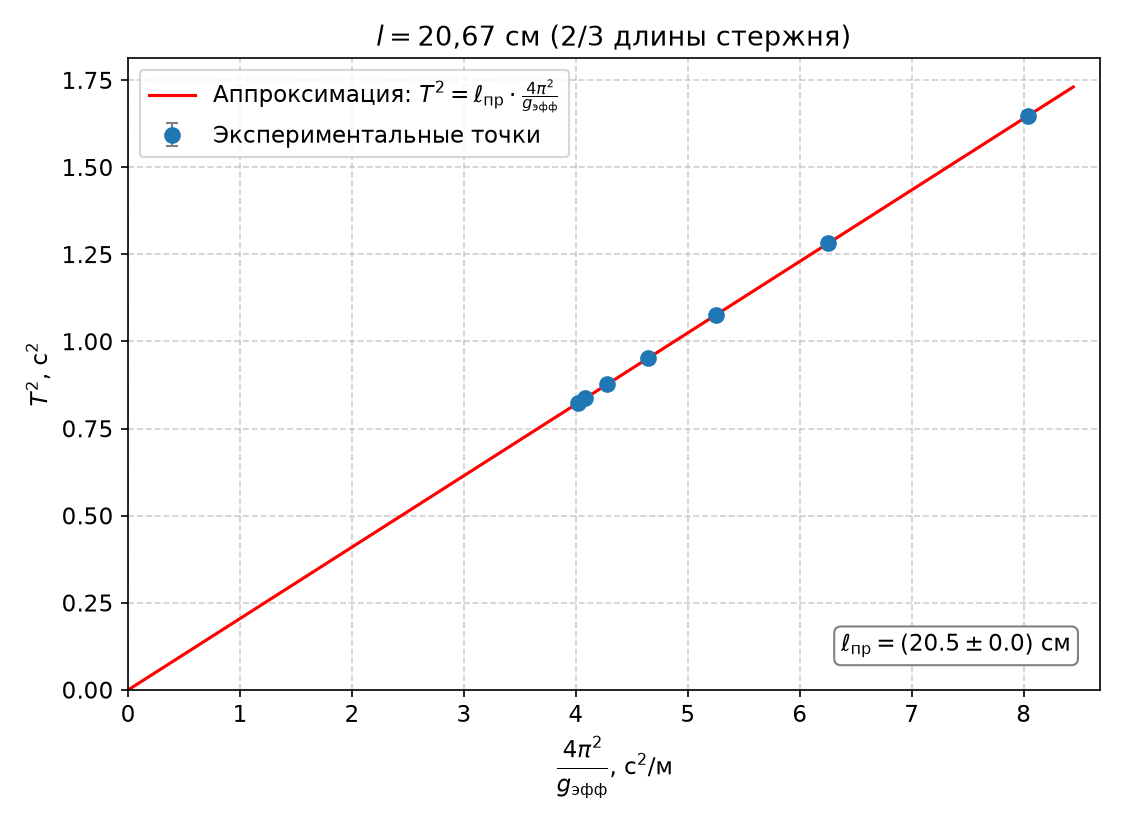
\includegraphics[width=0.8\textwidth]{assets/graph1.png}}
    \caption{Зависимость $T^2$ от $4\pi^2/g_{\text{эфф}}$ для $l = 20.67$ см}
    \label{fig:graph1}
\end{figure}

\begin{figure}[H]
    \centering
    \fbox{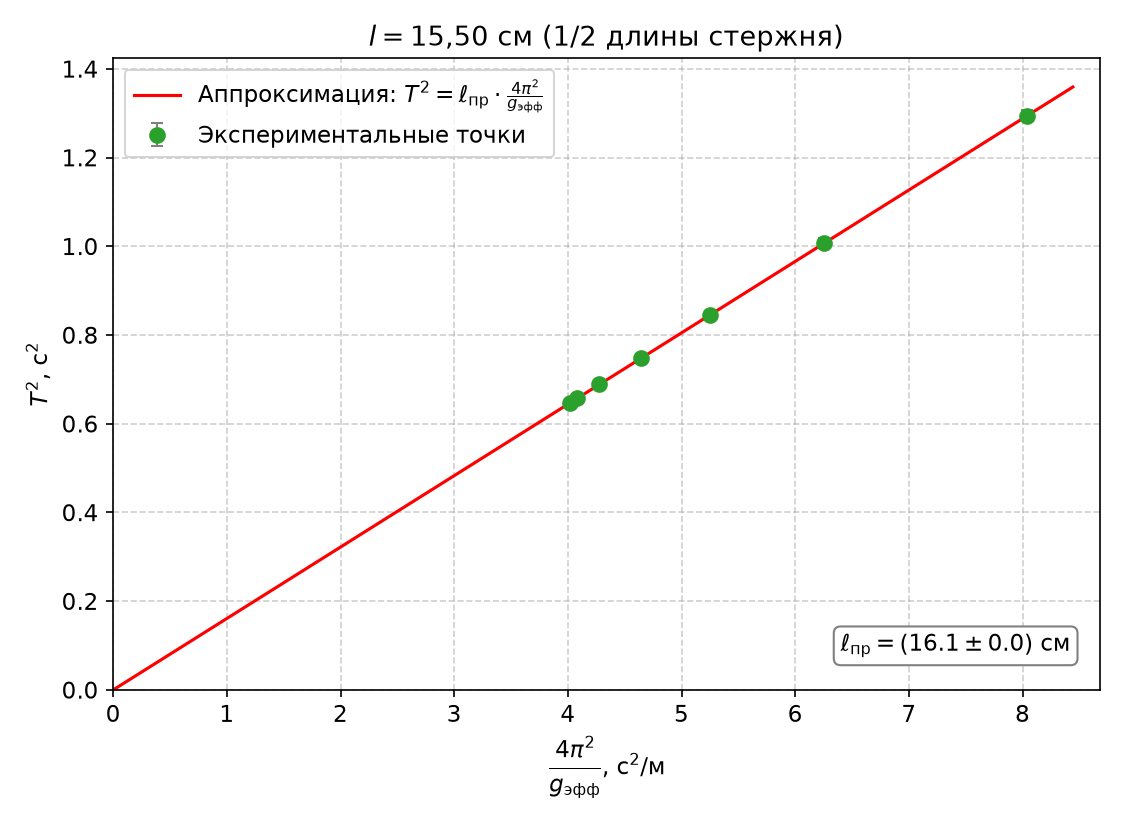
\includegraphics[width=0.8\textwidth]{assets/graph2.png}}
    \caption{Зависимость $T^2$ от $4\pi^2/g_{\text{эфф}}$ для $l = 15.50$ см}
    \label{fig:graph2}
\end{figure}

\begin{figure}[H]
    \centering
    \fbox{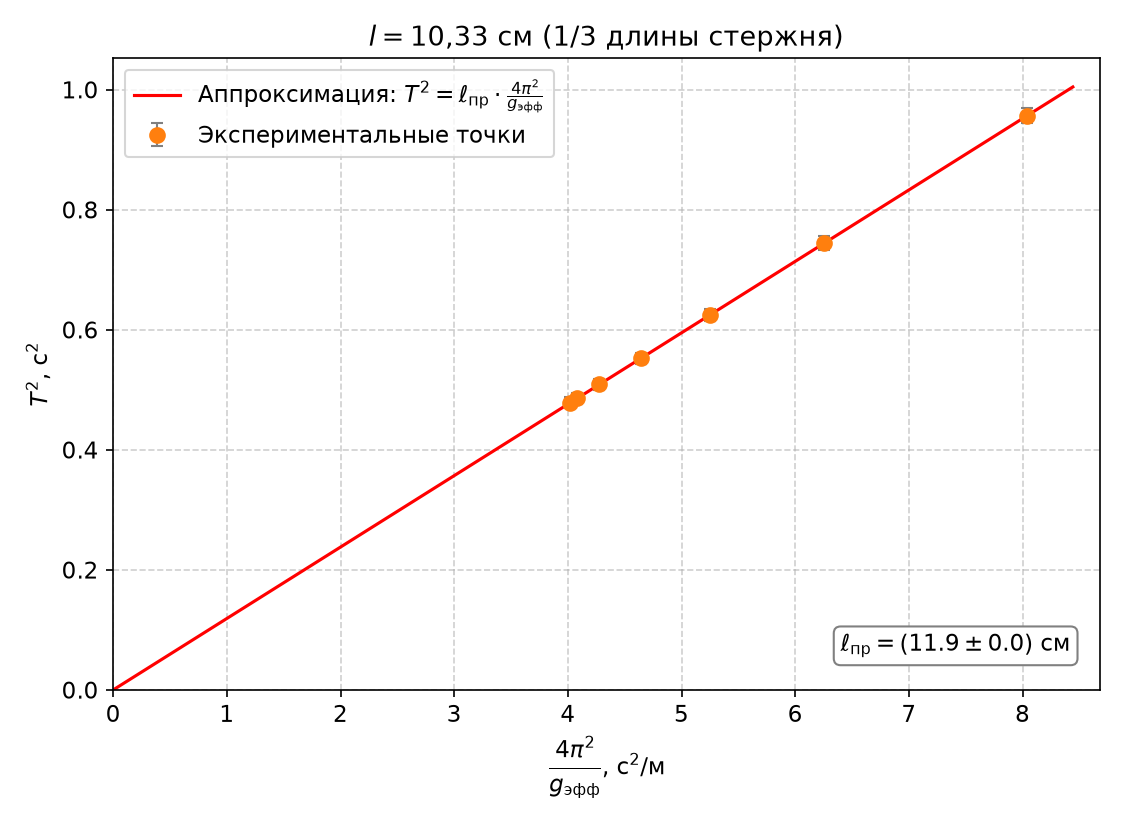
\includegraphics[width=0.8\textwidth]{assets/graph3.png}}
    \caption{Зависимость $T^2$ от $4\pi^2/g_{\text{эфф}}$ для $l = 10.33$ см}
    \label{fig:graph3}
\end{figure}

\end{document}